% !TEX program = pdflatex
\documentclass[11pt]{article}
\setlength{\textwidth}{6.5in}
\setlength{\oddsidemargin}{0pt}
\setlength{\evensidemargin}{0pt}
\setlength{\textheight}{9in}
\setlength{\topmargin}{0pt}
\addtolength{\topmargin}{-\headheight}
\addtolength{\topmargin}{-\headsep}
\ifdefined\pdfpagewidth \pdfpagewidth=8.5in \pdfpageheight=11in \fi
\ifdefined\pagewidth \pagewidth=8.5in \pageheight=11in \fi
\usepackage{amsmath,amssymb}
\usepackage{array}
\usepackage{booktabs}
\usepackage[tableposition=top]{caption}
\usepackage{longtable}
\usepackage{enumitem}
\usepackage{tikz}
\usepackage{pgfplots}
\pgfplotsset{compat=1.18}
\emergencystretch=3em

% ---- notation ---------------------------------------------------------------
\newcommand{\um}{\,$\mu$m}
\newcommand{\kms}{km\,s$^{-1}$}
\newcommand{\mJyb}{mJy\,beam$^{-1}$}
\newcommand{\uJyb}{$\mu$Jy\,beam$^{-1}$}
\newcommand{\lnu}{erg\,s$^{-1}$\,Hz$^{-1}$}
\newcommand{\sci}[2]{#1\times10^{#2}}

% ---- front matter -----------------------------------------------------------
\title{Radio Emission at 144\,MHz and 3\,GHz\\ from the T8.5+T9.5 Binary WISE 0458+6434}
\author{Charles C. Norton}
\date{}

\begin{document}
\maketitle

\begin{abstract}
Electron-cyclotron maser emission from brown dwarfs measures the magnetic fields of
objects too cold for any other magnetic diagnostic, and low frequencies reach fields of
tens of gauss. The third data release of the LOFAR Two-metre Sky Survey (LoTSS-DR3)
holds a component of $1.17\pm0.18$\,mJy at 144\,MHz $0.88''$ from the T8.5+T9.5 binary
WISEPC J045853.89+643452.9 (WISE 0458+6434) at $9.4$\,pc, where a component that bright
falls that close to any of the $64$ T and Y dwarfs DR3 covers with probability $0.003$.
In DR3's per-pointing images of five epochs from 2022 December to 2023 August the
circular polarisation at the binary's position is $-0.395\pm0.085$\,\mJyb\ ($-4.6\sigma$),
about $42$ per cent of the total intensity and the same within the errors at every epoch,
where $16$ compact sources of the same field read a fractional circular polarisation of
$+0.003$ and $+0.011$. The quick-look images of the VLA Sky Survey hold a $3$\,GHz source
of $472$--$634$\,\uJyb\ ($3.9$--$5.4\sigma$) within $0.54''$ of the binary's position on
each of 2017 October 11, 2023 February 9 and 2025 September 6, across the $2.8''$ the
binary moved, and nothing on 2020 August 25, where a source as bright would stand at
$3.4\sigma$ or more; the three positions fit the
binary's track ($\chi^2=1.3$ for $6$ degrees of freedom) and reject a fixed source
($\chi^2=16.1$ for $4$, $p=0.003$). The spectral luminosities, $\sci{1.2}{14}$\,\lnu\ at
$144$\,MHz and $\sci{5}{13}$ to $\sci{7}{13}$\,\lnu\ at $3$\,GHz, the strong circular
polarisation and the brightness temperature are those of auroral electron-cyclotron
emission, which at $3$\,GHz requires a field of about $1.1$\,kG where it forms. Both
components are later than the T8 dwarf WISE J062309.94$-$045624.6, the coldest brown
dwarf detected at radio wavelengths before.
\end{abstract}

% =============================================================================
\section{Introduction}\label{sec:intro}
% =============================================================================

Ultracool dwarfs, from the bottom of the main sequence down through the brown dwarfs,
carry magnetic fields of kilogauss strength, which they show through radio emission:
electrons accelerated along
the field lines of a large-scale magnetosphere radiate by the electron-cyclotron maser
instability at the local electron gyrofrequency, $\nu=2.8\,B$\,MHz for $B$ in gauss,
producing bright, strongly circularly polarised and often periodic emission, the radio
counterpart of the aurorae that the same currents drive~\cite{Treumann2006,Hallinan2015}.
At $4$--$8$\,GHz this emission has been found from late L and T dwarfs with fields above
$2.5$\,kG~\cite{Kao2016}, and Arecibo saw sporadic polarised flares from the T6.5 dwarf
2MASS J1047+21~\cite{RouteWolszczan2012}. The coldest brown dwarf detected at radio
wavelengths is the T8 dwarf WISE J062309.94$-$045624.6, whose periodic emission the
Australian Square Kilometre Array Pathfinder found~\cite{Rose2023}. Three Y dwarfs
observed at $4$--$8$\,GHz with the Jansky VLA gave no detection~\cite{Kao2019}, and a
search of the VLA Sky Survey (VLASS) catalogues and images at $14915$ ultracool dwarf
candidates of types M7.5 to L4 found no counterpart~\cite{Perger2025}.

Frequencies near $144$\,MHz probe fields near $50$\,G, which a gigahertz search cannot
see. The LOFAR Two-metre Sky Survey (LoTSS) found the T6.5 dwarf BDR J1750+3809 from its
circularly polarised emission before it was known as a brown dwarf~\cite{Vedantham2020},
and the T5.5+T7 binary WISEP J101905.63+652954.2 the same way, pulsing with a period of
about three hours~\cite{Vedantham2023}, with a field of about $126$\,G at its poles from the cutoff of
its radio spectrum~\cite{Yiu2026}. The circularly polarised catalogue of the second data
release held no other ultracool dwarf~\cite{Callingham2023}. The third data release
(DR3) extends the survey over the northern sky~\cite{Shimwell2026}, and this note reports
its detection of a T dwarf later than any of these, together with that source's circular
polarisation in DR3's per-pointing images and its $3$\,GHz counterpart in the VLASS
quick-look images.

\subsection{Contributions}
\begin{enumerate}[leftmargin=*,itemsep=1pt]
\item A search of LoTSS-DR3 at the T and Y dwarfs of the $20$\,pc census north of the
equator, which finds one, WISE 0458+6434.
\item The source's Stokes~V in the per-pointing images of the five DR3 epochs covering it,
read from the survey's archives by byte range, against the field's compact sources and
random positions.
\item Its $3$\,GHz counterpart in three of the four VLASS epochs, moving with the binary.
\end{enumerate}

% =============================================================================
\section{WISE 0458+6434}\label{sec:target}
% =============================================================================

WISEPC J045853.89+643452.9 was the first ultracool brown dwarf the Wide-field Infrared
Survey Explorer found~\cite{Mainzer2011}. Keck laser guide star adaptive optics resolved
it into two components $0.51''$ apart at position angle $320^\circ$, with estimated
temperatures near $600$ and $500$\,K~\cite{Gelino2011}, and resolved spectroscopy
classifies them T8.5 and T9.5, at the boundary between the T and Y classes, with ammonia
absorption in the secondary~\cite{Burgasser2012}. The $20$\,pc census gives a parallax
of $106.7$\,mas, a distance of $9.37$\,pc and so a projected separation of $4.8$\,au, and
a proper motion of $210.4$\,mas\,yr$^{-1}$ east and $289.6$\,mas\,yr$^{-1}$ north,
$358$\,mas\,yr$^{-1}$ at position angle $36^\circ$~\cite{Kirkpatrick2021}. Positions in
this note are carried from the census's position at epoch 2016.45 along that motion.

% =============================================================================
\section{Data and method}\label{sec:method}
% =============================================================================

\paragraph{The DR3 component catalogue.} The $156$ objects of the Gaia Catalogue of
Nearby Stars within $10$\,pc and the $80$ T and Y dwarfs of the $20$\,pc census north of
the equator were carried to 2019.5 and matched to the DR3 component catalogue (VizieR
J/A+A/707/A198) within $3''$, the same positions moved $2'$ in four directions serving as
the null. The chance of a match follows from DR3's local density of components.

\paragraph{The per-pointing images.} The DR3 mosaic at a position combines several
pointings, each an $8$\,h observation of one epoch. The ASTRON VO's table of DR3
pointings gives their dates, and the SURF Data Repository holds each pointing's products
as tar archives of $10$--$23$\,GB, from which the $6''$ Stokes~I image with astrometric
corrections and the $6''$ dirty Stokes~I and V images were read by HTTP byte range, a
patch around the target alone. Each pointing's images are put on DR3's flux scale by the
factor the release gives for that pointing. Stokes~V is read at the binary's position on
the pointing's date, its noise from the robust scatter of the annulus $12''$--$30''$ out,
and epochs are combined by inverse variance. The field's other compact sources and
random positions in the same images are the null.

\paragraph{VLASS.} The quick-look images of the four VLASS epochs~\cite{Lacy2020} come
from the Canadian Astronomy Data Centre as cutouts. In each, the brightest pixel within
$2.5''$ of the binary's position on the image's date is set against the image's robust
noise, a Gaussian fitted to it gives its offset, and the same statistic at $2000$ random
positions $15''$--$150''$ away gives the rate at which noise alone reaches it. Quick-look
positions carry systematic errors of about $0.5''$~\cite{Gordon2021}, which are added in
quadrature to the fitted errors.

% =============================================================================
\section{Results}\label{sec:results}
% =============================================================================

\subsection{The 144 MHz source}

Of the $126$ stars within $10$\,pc inside DR3's coverage, $7$ carry a component within
$3''$, against $0.25$ at the moved positions: the flare stars YZ~CMi, AD~Leo, EV~Lac,
EQ~Peg, V374~Peg and the pair GJ~1116~A and B. Of the $64$ T and Y dwarfs inside the
coverage, one does, against $0.00$ moved. WISE 0458+6434 lies under a component of
$1.17\pm0.18$\,mJy with a peak of $0.90$\,\mJyb\ (signal-to-noise ratio $11$),
unresolved at $7.6''\times6.1''$, $0.88''$ from the binary's 2019.5 position at position
angle $45^\circ$, against the proper motion's $36^\circ$: the DR3 epochs fall in 2022 and
2023, and the binary had moved $1.2''$ to $1.5''$ along that direction by then. DR3's
local density of $275$ components above $1$\,mJy per square degree puts a component that
bright within $0.88''$ of any of the $64$ dwarfs with probability $0.003$. Nothing lies
within $10''$ in NVSS, the VLASS epoch-1 component catalogue, WENSS, Pan-STARRS1 or Gaia,
and AllWISE's only source there is the binary.

\subsection{Circular polarisation}

Table~\ref{tab:lofar} gives the five pointings whose images cover the binary. In the two
nearest the pointing centre, P078+64 of 2022 December 29 and P072+64 of 2023 July 14, the
restored Stokes~I image holds the source at signal-to-noise ratios of $10.8$ and $4.6$,
$0.36''$ and $0.98''$ from the binary's position on each date, with Stokes~V at the
Stokes~I peak of $-0.383\pm0.118$ and $-0.253\pm0.116$\,\mJyb\ before the flux scale,
fractions of $-0.44\pm0.14$ and $-0.43\pm0.23$ of the dirty Stokes~I there. The $16$
other compact sources of $1.1$--$6.8$\,\mJyb\ within $10.5'$ give median fractions of
$+0.003$ and $+0.011$ in the two epochs, none beyond $2.7\sigma$; no pixel of the two
epochs' combined Stokes~V map more than $30''$ from the binary reaches $4.7\sigma$ of
either sign among about $33800$ beams; and at $195419$ random positions both epochs reach
the binary's values with one sign at a rate of $\sci{2}{-5}$.

All five epochs on DR3's flux scale give $-0.395\pm0.085$\,\mJyb\ at the binary's
position ($-4.6\sigma$), with $\chi^2=2.4$ for $4$ degrees of freedom about that value,
and Stokes~I of $0.93\pm0.11$\,\mJyb, a fractional polarisation of about $-0.42$. A
reading of the same images through the two nearest pointings, part of a survey of the
nearest stars, gives $-4.1\sigma$. Among the $1631$ objects SIMBAD lists as brown dwarfs
north of $-1^\circ$ that DR3's per-pointing images measure, two exceed $3.5\sigma$ in
Stokes~V: WISE 0458+6434 and WISEP J101905.63+652954.2 ($-3.8\sigma$), the binary LOFAR
found before~\cite{Vedantham2023}. The Stokes~I peak of the two deepest epochs differs by
a factor of $0.46\pm0.11$ against $0.83\pm0.14$ for the field's sources, a difference of
$2\sigma$.

\begin{table}[t]
\centering\small
\caption{WISE 0458+6434 in the per-pointing images of LoTSS-DR3: the pointing, its date,
the binary's distance from the pointing centre, DR3's flux-scale factor, the dirty
Stokes~I peak within $4.5''$ of the binary and Stokes~V at the binary's position, both
scaled. The low-S/N peaks are biased upward by the search for a maximum.}
\label{tab:lofar}
\begin{tabular}{llrrrr}
\toprule
Pointing & Date & Offset ($^\circ$) & Scale & $I$ (\mJyb) & $V$ (\mJyb) \\
\midrule
P072+67 & 2022 Dec 28 & $2.34$ & $1.159$ & $0.60\pm0.31$ & $-0.13\pm0.25$ \\
P078+64 & 2022 Dec 29 & $1.62$ & $1.052$ & $1.25\pm0.19$ & $-0.40\pm0.13$ \\
P072+64 & 2023 Jul 14 & $1.09$ & $1.181$ & $0.74\pm0.16$ & $-0.39\pm0.14$ \\
P075+62 & 2023 Aug 19 & $2.93$ & $0.991$ & $1.32\pm0.55$ & $-0.71\pm0.53$ \\
P078+67 & 2023 Aug 20 & $2.66$ & $1.132$ & $1.00\pm0.39$ & $-0.69\pm0.32$ \\
\midrule
Combined & & & & $0.93\pm0.11$ & $-0.395\pm0.085$ \\
\bottomrule
\end{tabular}
\end{table}

The visibilities of the 2023 July 14 observation ($25$ sub-bands, $56.6$\,GB) were read
from the archive and phase-rotated to the binary, to four positions $45''$ away and to a
$7.78$\,mJy source of the field. Without the archive's direction-dependent calibration
solutions, the check source keeps about a tenth of its flux, and the binary's Stokes~V
series binned from $8$\,s to $30$\,min holds no excursion beyond $4\sigma$ of the offset
positions' scatter and no period between $0.5$ and $4$\,h (false-alarm probability
$0.60$). At that calibration a burst would have to reach of order $100$\,mJy for a minute
to show.

\subsection{The 3 GHz source}

Table~\ref{tab:vlass} and Figure~\ref{fig:track} give the VLASS epochs. In 2017, 2023
and 2025 the brightest pixel within $2.5''$ of the binary stands at $3.9$--$5.4\sigma$,
$0.23''$--$0.54''$ from the binary's position on the date, a level that $2000$ random
positions in the same images reach once in the three epochs; in 2020 the binary's
position holds nothing ($0.1\sigma$, a $5\sigma$ limit of $0.7$\,mJy). Over the eight
years the binary moved $2.8''$. The three positions, with the fitted and systematic
errors in quadrature, give $\chi^2=1.3$ for $6$ degrees of freedom about the binary's
track and $\chi^2=16.1$ for $4$ about the best fixed position ($p=0.003$), so the source
moves with the binary; the two LOFAR positions of 2022--2023 lie on the track as well,
the five together giving $\chi^2=12.1$ for $10$ about the track and $18.8$ for $8$ about
a fixed position.

\begin{table}[t]
\centering\small
\caption{WISE 0458+6434 in the VLASS quick-look images: the epoch, the date, the beam,
the brightest pixel within $2.5''$ of the binary's position on the date and its
signal-to-noise ratio, the fitted position's offset east and north of the binary, and
the share of $2000$ random positions where the same statistic is as high.}
\label{tab:vlass}
\begin{tabular}{llcrrcr}
\toprule
Epoch & Date & Beam ($''$) & Peak (\uJyb) & S/N & Offset E, N ($''$) & Random \\
\midrule
1.1 & 2017 Oct 11 & $3.1\times2.1$ & $634$ & $5.4$ & $+0.07$, $-0.32$ & $0.0000$ \\
2.1 & 2020 Aug 25 & $3.3\times2.1$ & $13$ & $0.1$ & -- & -- \\
3.1 & 2023 Feb 9 & $2.6\times2.2$ & $477$ & $4.3$ & $+0.00$, $-0.23$ & $0.0000$ \\
4.1 & 2025 Sep 6 & $2.6\times2.0$ & $472$ & $3.9$ & $+0.54$, $-0.02$ & $0.0005$ \\
\bottomrule
\end{tabular}
\end{table}

\begin{figure}[t]
\centering
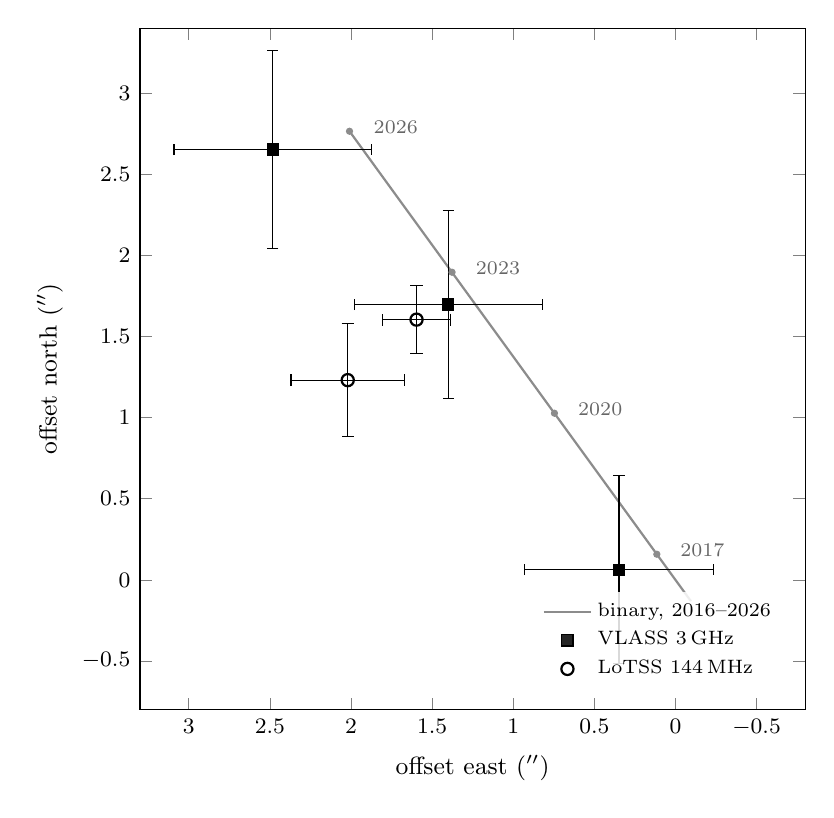
\begin{tikzpicture}
\begin{axis}[width=0.62\textwidth,height=0.62\textwidth,axis equal image,
  xmin=-0.8,xmax=3.3,ymin=-0.8,ymax=3.4,x dir=reverse,
  xlabel={offset east ($''$)},ylabel={offset north ($''$)},
  tick label style={font=\footnotesize},label style={font=\small},
  legend style={font=\scriptsize,at={(0.97,0.03)},anchor=south east,draw=none,fill=white,fill opacity=0.85,text opacity=1},legend cell align=left]
\addplot[black!45,thick] coordinates {(-0.095,-0.131) (2.009,2.765)};
\addlegendentry{binary, 2016--2026}
\addplot[only marks,mark=*,mark size=1.1pt,black!45,forget plot] coordinates {(0.115,0.158) (0.746,1.027) (1.377,1.896) (2.009,2.765)};
\node[font=\scriptsize,text=black!60,anchor=west] at (axis cs:0.03,0.18) {2017};
\node[font=\scriptsize,text=black!60,anchor=west] at (axis cs:0.66,1.05) {2020};
\node[font=\scriptsize,text=black!60,anchor=west] at (axis cs:1.29,1.92) {2023};
\node[font=\scriptsize,text=black!60,anchor=west] at (axis cs:1.92,2.79) {2026};
\addplot[only marks,mark=square*,mark size=2pt,black,error bars/.cd,x dir=both,x explicit,y dir=both,y explicit]
  coordinates {(0.348,0.063) +- (0.58,0.58) (1.400,1.697) +- (0.58,0.58) (2.481,2.652) +- (0.61,0.61)};
\addlegendentry{VLASS 3\,GHz}
\addplot[only marks,mark=o,mark size=2.2pt,black,thick,error bars/.cd,x dir=both,x explicit,y dir=both,y explicit]
  coordinates {(1.596,1.604) +- (0.21,0.21) (2.020,1.231) +- (0.35,0.35)};
\addlegendentry{LoTSS 144\,MHz}
\end{axis}
\end{tikzpicture}
\caption{Positions of the radio source relative to WISE 0458+6434's position at epoch
2016.45, east to the left. The line is the binary's track from 2016 to 2026, marked at
2017, 2020, 2023 and 2026; the squares are the VLASS detections of 2017, 2023 and 2025
and the circles the two deepest LoTSS-DR3 epochs, of 2022 December and 2023 July, each
with its fitted and systematic errors in quadrature.}
\label{fig:track}
\end{figure}

% =============================================================================
\section{Discussion}\label{sec:discussion}
% =============================================================================

At $9.37$\,pc the $144$\,MHz flux density corresponds to a spectral luminosity of
$\sci{1.2}{14}$\,\lnu, of which $\sci{4}{13}$\,\lnu\ is circularly polarised, and the
VLASS detections to $\sci{5.0}{13}$--$\sci{6.7}{13}$\,\lnu\ at $3$\,GHz. Emission from a
region of radius $R$ at $144$\,MHz has a brightness temperature of
$\sci{1}{13}\,(R/R_\mathrm{J})^{-2}$\,K, above the $10^{12}$\,K that incoherent
synchrotron emission reaches for any region smaller than about three Jupiter radii, and a
circular polarisation of $42$ per cent at $144$\,MHz is not that of gyrosynchrotron
emission from an optically thick region. Both point to the electron-cyclotron maser,
which emits near the local gyrofrequency: $144$\,MHz needs about $51$\,G where it forms
and $3$\,GHz about $1.1$\,kG, or half these at the second harmonic. A surface field of a
kilogauss or more on one of the components, which $4$--$8$\,GHz detections have shown
in T dwarfs before~\cite{Kao2016}, would supply both frequencies from heights of about
three radii and from near the surface. In 2020 the binary's position reads
$13$\,\uJyb\ against a noise of $140$\,\uJyb, where a source as bright as in the other
epochs would stand at $3.4$--$4.5\sigma$, as the emission's beaming across the rotation
or its variability from epoch to epoch would make it in the seconds-long VLASS
snapshots; the $144$\,MHz polarisation is the same within its errors over the five
$8$\,h epochs.

The two components lie $0.51''$ apart, unresolved by either survey, so the emitter is
not identified. Both are later than the T8 dwarf WISE J062309.94$-$045624.6, the
coldest brown dwarf detected at radio wavelengths before~\cite{Rose2023}, and at
T8.5+T9.5 the binary is the latest-type brown dwarf system detected at any radio
frequency and the first at the boundary of the T and Y classes. The orbit of about
$70$\,yr~\cite{Gelino2011} is too wide for the components' magnetospheres to interact,
so the emission is each dwarf's own.

The chance that an unrelated source accounts for the detection is small on each count:
$0.003$ for a $144$\,MHz component that close among the $64$ dwarfs, $\sci{2}{-5}$ for
Stokes~V of the observed strength and sign at a random position in both deep epochs, and
$0.003$ for the VLASS positions under a fixed source, which also leaves the binary's
motion between 2017 and 2025 unexplained. A background active galaxy would carry a
circular polarisation below one per cent, as the field's $16$ compact sources do.

% =============================================================================
\section{Related work}\label{sec:related}
% =============================================================================

The radio emission of brown dwarfs has been found mostly by targeted gigahertz
observations~\cite{RouteWolszczan2012,Kao2016,Rose2023}, and at $144$\,MHz by the LoTSS
search for circularly polarised sources~\cite{Vedantham2020,Vedantham2023,Callingham2023}.
The VLASS search of ultracool dwarfs found none~\cite{Perger2025}; its sample was the
M7.5 to L4 candidates of a catalogue built on Gaia DR2, which holds no T dwarfs, and the
VLASS epoch-1 component catalogue does not list the 2017 source here. The VLA observations of three
Y dwarfs reached $2$--$7$\,$\mu$Jy rms at $4$--$8$\,GHz without a
detection~\cite{Kao2019}. No earlier radio detection of WISE 0458+6434 is found in the
literature.

% =============================================================================
\section{Conclusion}\label{sec:conclusion}
% =============================================================================

WISE 0458+6434, a T8.5+T9.5 binary at $9.4$\,pc, emits at $144$\,MHz with a circular
polarisation of about $42$ per cent over five epochs of 2022--2023 and at $3$\,GHz in
three of four VLASS epochs from 2017 to 2025, the $3$\,GHz source moving with the binary.
The luminosity, polarisation and brightness temperature are those of auroral
electron-cyclotron emission, which at $3$\,GHz requires a field of about a kilogauss
where it forms, and the binary is the latest-type brown dwarf system detected at radio
wavelengths. Time-resolved observations at either frequency would give the emitter's
rotation period through its pulses, the polarisation at $3$\,GHz would fix the
emission's mode, and resolved observations would identify the component.

\section*{Acknowledgements}

This work uses LoTSS-DR3 data from the LOFAR telescope, designed and constructed by
ASTRON, with its products served by the ASTRON VO and the SURF Data Repository; the VLA
Sky Survey of the National Radio Astronomy Observatory, a facility of the National
Science Foundation operated by Associated Universities, Inc., with quick-look images
served by the Canadian Astronomy Data Centre; and the SIMBAD and VizieR services and the
XMatch service at CDS, Strasbourg.

\begin{thebibliography}{99}\small\raggedright
\setlength{\itemsep}{1pt}

\bibitem{Treumann2006}
R.~A. Treumann, The electron-cyclotron maser for astrophysical application,
\emph{Astron. Astrophys. Rev.} \textbf{13}, 229 (2006).

\bibitem{Hallinan2015}
G.~Hallinan, S.~P. Littlefair, G.~Cotter, et al., Magnetospherically driven optical and
radio aurorae at the end of the stellar main sequence, \emph{Nature} \textbf{523}, 568
(2015).

\bibitem{Kao2016}
M.~M. Kao, G.~Hallinan, J.~S. Pineda, et al., Auroral radio emission from late L and T
dwarfs: a new constraint on dynamo theory in the substellar regime, \emph{Astrophys. J.}
\textbf{818}, 24 (2016).

\bibitem{RouteWolszczan2012}
M.~Route and A.~Wolszczan, The Arecibo detection of the coolest radio-flaring brown
dwarf, \emph{Astrophys. J. Lett.} \textbf{747}, L22 (2012).

\bibitem{Rose2023}
K.~Rose, J.~Pritchard, T.~Murphy, et al., Periodic radio emission from the T8 dwarf
WISE J062309.94$-$045624.6, \emph{Astrophys. J. Lett.} \textbf{951}, L43 (2023).

\bibitem{Kao2019}
M.~M. Kao, G.~Hallinan and J.~S. Pineda, Constraints on magnetospheric radio emission
from Y dwarfs, \emph{Mon. Not. R. Astron. Soc.} \textbf{487}, 1994 (2019).

\bibitem{Perger2025}
K.~Perger, B.~Seli and K.~Vida, Radio emission from flaring stars and brown dwarfs,
\emph{Astron. Astrophys.} \textbf{699}, A337 (2025).

\bibitem{Vedantham2020}
H.~K. Vedantham, J.~R. Callingham, T.~W. Shimwell, et al., Direct radio discovery of a
cold brown dwarf, \emph{Astrophys. J. Lett.} \textbf{903}, L33 (2020).

\bibitem{Vedantham2023}
H.~K. Vedantham, T.~J. Dupuy, E.~L. Evans, et al., Polarised radio pulsations from a new
T dwarf binary, \emph{Astron. Astrophys.} \textbf{675}, L6 (2023).

\bibitem{Yiu2026}
T.~W.~H. Yiu, H.~K. Vedantham, J.~R. Callingham and T.~W. Shimwell, The magnetic field
strength of a methane dwarf measured from its radio spectral cutoff, arXiv:2607.19642
(2026).

\bibitem{Callingham2023}
J.~R. Callingham, T.~W. Shimwell, H.~K. Vedantham, et al., V-LoTSS: the circularly
polarised LOFAR Two-metre Sky Survey, \emph{Astron. Astrophys.} \textbf{670}, A124
(2023).

\bibitem{Shimwell2026}
T.~W. Shimwell, M.~J. Hardcastle, C.~Tasse, et al., The LOFAR Two-metre Sky Survey: VII.
Third data release, \emph{Astron. Astrophys.} \textbf{707}, A198 (2026).

\bibitem{Mainzer2011}
A.~Mainzer, M.~C. Cushing, M.~Skrutskie, et al., The first ultra-cool brown dwarf
discovered by the Wide-field Infrared Survey Explorer, \emph{Astrophys. J.} \textbf{726},
30 (2011).

\bibitem{Gelino2011}
C.~R. Gelino, J.~D. Kirkpatrick, M.~C. Cushing, et al., WISE brown dwarf binaries: the
discovery of a T5+T5 and a T8.5+T9 system, \emph{Astron. J.} \textbf{142}, 57 (2011).

\bibitem{Burgasser2012}
A.~J. Burgasser, C.~R. Gelino, M.~C. Cushing and J.~D. Kirkpatrick, Resolved
spectroscopy of a brown dwarf binary at the T dwarf/Y dwarf transition,
\emph{Astrophys. J.} \textbf{745}, 26 (2012).

\bibitem{Kirkpatrick2021}
J.~D. Kirkpatrick, C.~R. Gelino, J.~K. Faherty, et al., The field substellar mass
function based on the full-sky 20 pc census of 525 L, T, and Y dwarfs,
\emph{Astrophys. J. Suppl.} \textbf{253}, 7 (2021).

\bibitem{Lacy2020}
M.~Lacy, S.~A. Baum, C.~J. Chandler, et al., The Karl G. Jansky Very Large Array Sky
Survey (VLASS): science case and survey design, \emph{Publ. Astron. Soc. Pac.}
\textbf{132}, 035001 (2020).

\bibitem{Gordon2021}
Y.~A. Gordon, M.~M. Boyce, C.~P. O'Dea, et al., A quick look at the 3 GHz radio sky. I.
Source statistics from the Very Large Array Sky Survey, \emph{Astrophys. J. Suppl.}
\textbf{255}, 30 (2021).

\end{thebibliography}

\end{document}
